
%===============%                               %~~~~~~~~~~~~~~~~~~~~~~~~~~~~~~~~~~~~~~~~~~~~~~~~~%
% DOCUMENTCLASS %                                See full option description in "mytemplate.cls"
%===============%                               %~~~~~~~~~~~~~~~~~~~~~~~~~~~~~~~~~~~~~~~~~~~~~~~~~%
 
\documentclass[
   UAM                                          % Document type (non-standard)
 , 12pt                                         % Text size
%  , draft
%  , final                                        % Quality
 , xelatex                                      % Use the XeLaTeX compiler
%  , biblatex                                     % Use 'biblatex' for references (best by far)
 , bibtex                                       % Use 'bibtex' for references (oldschool :)
%  , movie
%  , notodos                                      % Disable todos
 , layout
%  , defaultformat                                % Attempt to use default formatting options
%  , glossary                                     % Use a glossary
]{common/mytemplate}

% \bibliography{references}
\hypersetup{
   bookmarksopen=true
 , bookmarksopenlevel=2
}
% Load the references.bib file
% \bibliography{references}

\newlength\oldparindent
\setlength\oldparindent{\parindent}

\newlength\figwidth
\setlength\figwidth{0.7\linewidth}

% \setlength\floatsep{\baselineskip}
\setcounter{topnumber}{1}
% \setlength\baselineskip{12pt}
% \selectfont
\begin{document}

\pagestyle{plain}
% \layout
% \printinunitsof{cm}
% \prntlen{\baselineskip}
% \the\textwidth
% \the\linewidth
% \prntlen{\textwidth}\\
% \prntlen\linewidth\\
% \prntlen\oddsidemargin\\
% \prntlen\oddsidemargin
% \newpage



\title{A Low Complexity Adaptive Beamformer\\for Active Sonar Imaging}%
%
\author{J.I.Buskenes\firstAddress, A.Austeng\firstAddress, C.-I.C.Nilsen\firstAddress}%
%
\begin{contact}
  \firstAddress Dept. of Informatics, P.Box 1080 Blindern, N-0316 OSLO
\end{contact}%
%
\begin{contact}
Contact author: Jo Inge Buskenes\\
Dept. of Informatics, Univ. of Oslo, P.Box 1080 Blindern, N-0316 OSLO\\
\href{mailto:joibu@ifi.uio.no}{joibu@ifi.uio.no}
\end{contact}%
%
\begin{abstract}
The angular resolution and contrast in active sonar images depend on the beamformer's ability to receive signals from directions of interest, while suppressing noise and interference emanating from other directions. For sonar arrays, this is achieved by applying weights to the array channels.

While classical beamformers use predefined windows, adaptive beamformers estimate the optimal window by analytical evaluation of the data. The minimum variance (MV) beamformer, for instance, calculates the set of weights that minimises the variance of the beamformer's output. 

We have implemented a Low Complexity Adaptive (LCA) beamformer, which adaptively selects a window from a predefined set. The set is comprised of windows that are typical solutions found by the Minimum Variance method. The LCA beamformer was tested using simulated and experimental data from the Kongsberg Maritime HISAS 1030 sonar. On a simulated scene with speckle, highlight and shadow, the beamformer offered better lateral edge definition compared to the MV beamformer, and speckle intensity and shape comparable to DAS and MV beamformers. These results were verified by the experimental data.

An attactive trait of the LCA is its low computational complexity; while the MV beamformer is of O($M^3$), the LCA method is of O($MW$), with $M$ being the number of channels and $W$ the number of windows. We made the LCA perform like the MV method using a well designed set of 30 windows. Hence, unless the array is very small, the proposed method will perform like the MV beamformer or better, and at a fraction of the computational cost.
\end{abstract}%
%
\keywords{Beamforming, Capon, Minimum variance, Low Complexity, Sonar}

% \titlepage

\newpage
% \the\lineheight
\section{Introduction}

In active sonar array imaging, an acoustic wave is transmitted and the received echoes are usually recorded using an array of sensors. Each of these may be independently delayed and weighted such that signals emanating from directions of interest are added constructively, while noise and interference from other directions add destructively. Additionally, a window may be applied to the sensor channels to further adjust the arrays spatial response. This process is known as beamforming.% The process of combining the signals from each sensor is known as beamforming.

Traditional beamformers such as Delay-and-Sum (DAS) weight the sensors using a predefined window. However, since the optimal spatial response is likely to change with time, it is often preferred to use beamformers that continously adapt the weights to the dynamic data. This usually involves solving some optimization problem.

The Minimum Variance (MV) beamformer selects the window that minimizes the beamformer's output power~\cite{cap69}. It has recently been investigated for active sonar imaging in e.g.~\cite{saf09}, and in ultrasound imaging in e.g.~\cite{syn07}. We suggest using a Low Complexity Adaptive (LCA) beamformer, which for each pixel applies a set of predefined windows and selects one of them based on the MV criterion. Using the LCA beamformer results in increased robustness and improved edge definition compared to the MV and DAS beamformers.


% When the wavefield is sampled using an array of sensors, the data from each sensor may be 
% 
% Traditional beamformers such as Delay-and-Sum (DAS) apply predefined windows to all incoming data. However, due to the non-stationary nature of sonar data, the optimal window for any given time instant will generally differ from the next. This is where adaptive beamformers thrive, because they compute the optimal window coefficients for the data at each time instant. The choice of optimisation criteria is what mainly differentiates the various adaptive beamformers. The Minimum Variance (MV) beamformer, for instance, selects the set of weights that minimizes the beamformer output power for any given time instant~\cite{cap69}.


\section{Background}

% Adaptive beamformers usually compute the window coefficients by estimating and inverting a spatial covariance matrix. There are two inherent problems to this procedure. First, for improved estimation accuracy the data is either averaged in space or time, and the significance of the covariance matrix can be reduced using a regularisation parameter~\cite{Carl Inge}. These are all attempts to constrain the beamformer to ensure the window coefficience are not over-adapted to the data. Second, inverting the covariance matrix has a computational complexity of O($M^3$)~\cite{Carl Inge}. For larger arrays the computational burden becomes significant, and the question arises whether this processing power can be better utilised. 

The MV beamformer computes the window coefficients by estimating and inverting a spatial covariance matrix. For improved estimation accuracy the data is averaged in space or time, or both. In addition, a certain amount of diagonal loading is often added to the covariance matrix before inversion. These actions, while leading to statistical robustness, tend to deteriorate the beamformer's performance. Also, the inversion of the covariance matrix has a computational complexity of O($M^3$), where $M$ is the number of elements. The computational burden makes the MV beamformer for large arrays less attractive, and sometimes even infeasible.

Based on the proposed method by Synnevåg~\cite{syn11}, we have implemented the LCA beamformer that keeps the minimum variance optimisation criterion but reduces the solution space to a discrete set of predefined windows. This reduces the computational complexity to O($MW$), where $W$ is the number of windows in the set. We use the Kaiser window function because it allows us to design a wide range of windows with different mainlobe widths and sidelobe suppression by adjusting the tradeoff parameter $\beta$~\cite{kai66}. In addition we apply steering to each of the windows and constrain the window design to ensure unit gain in the look direction.

The following will show that the proposed method performs similarly to or better than the MV method.

\begin{figure}[tp]\centering%
\subfigure{%
\graphicsAI[width=\linewidth]{gfx/img_das_lca_mv.pdf}}
\subfigure{%
\graphicsAI[width=\linewidth]{gfx/img_das_lca_mv_mean100.pdf}}%
\caption{A simulated circular object buried in speckle is imaged from above.\newline\parbox[t]{1.50cm}{Top:\newline Bottom:}\parbox[t]{6.8cm}{Image of a single speckle realisation.\newline Mean image of 100 speckle realisations.}}\label{speckle}%%
\end{figure}%
\begin{figure}[t]\centering%
\graphicsAI[width=\linewidth]{gfx/img_mean_cut.pdf}%
\caption{Lateral cut in the mean image at range 41.1\,m (highlight) and 44.5\,m (shadow).}\label{cutmean}%
\end{figure}
% \begin{figure}[t]\centering
% % \graphicsAI[drawing,width=\linewidth]{gfx/the_box.svg}\\
% 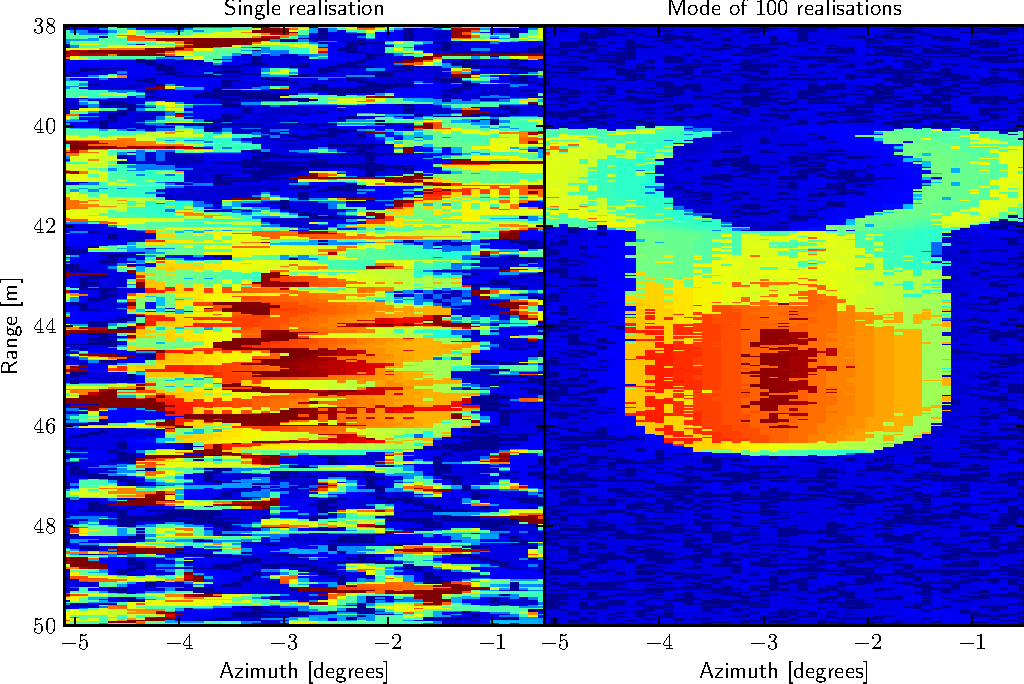
\includegraphics[width=\linewidth]{gfx/selected_windows.pdf}
% \caption{Selected windows}\label{selected_windows}
% \end{figure}
% \begin{figure}[t]\centering
% 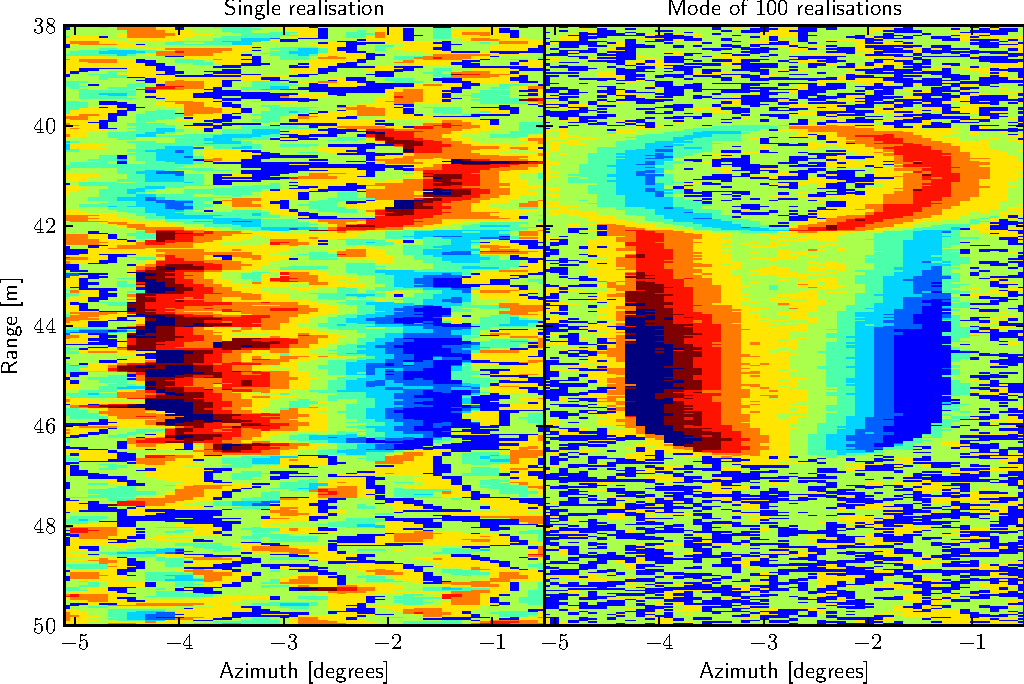
\includegraphics[width=\linewidth]{gfx/selected_windows_angle.pdf}
% \caption{Selected windows - Colored by angle}\label{selected_windows_angle}
% 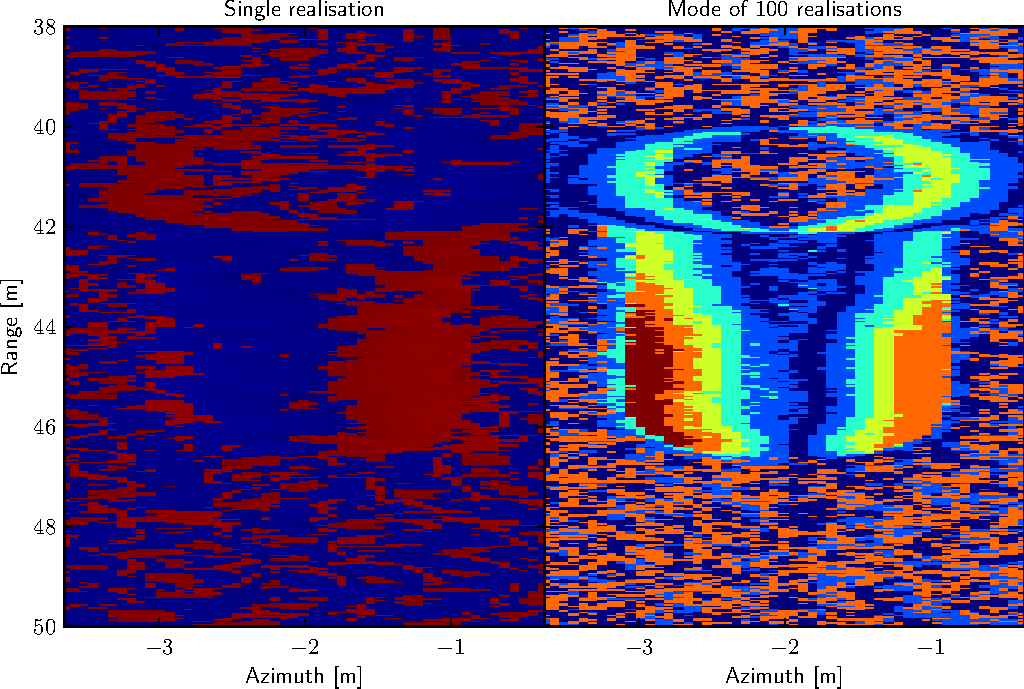
\includegraphics[width=\linewidth]{gfx/selected_windows_sym_angle.pdf}
% \caption{Selected windows - Colored symmetrically by angle}\label{selected_windows_sym}
% \end{figure}
\begin{figure}[t]\centering
\graphicsAI[width=\linewidth]{gfx/img_holmengraa.pdf}%
\caption{HISAS sidescan sonar (SSS) image of the shipwreck Holmengraa.}\label{holmengraa}%
\end{figure}

% Adaptive beamformers usually compute the window coefficients by estimating and inverting a spatial covariance matrix. There are two inherent problems to this procedure. First, for improved estimation accuracy the data is either averaged in space or time, and the significance of the covariance matrix can be reduced using a regularisation parameter~\cite{Carl Inge}. These are all attempts to constrain the beamformer to ensure the window coefficience are not over-adapted to the data. Second, inverting the covariance matrix has a computational complexity of O($M^3$)~\cite{Carl Inge}. For larger arrays the computational burden becomes significant, and the question arises whether this processing power can be better utilised. 
% 
% Based on the proposed method by Synnevåg~\cite{syn11}, we have implemented a Low Complexity Adaptive (LCA) beamformer that keeps the minimum variance optimisation criteria but reduces the solution space to a discrete set of predefined windows. We use the Kaiser window function because it allows us to design a wide range of windows with different mainlobe widths and sidelobe suppression by adjusting the tradeoff parameter $\beta$. In addition we apply steering $\varphi$ to each of the windows and and constrain the window design to ensure unit gain in the look direction.

\section{Experimental Setup}

For the LCA to perform well it is important to let it have a diverse selection of windows to choose from. This selection is based on observations of the solutions found by the MV beamformer. We obtained good results in our experiments by letting the LCA beamformer select among 5 Kaiser windows with uniformly distributed $\beta$'s in the range $[0.05, 0.5]$ and a rectangular window. Each window was steered in 5 different directions, uniformly distributed within 80\% of the mainlobe width of the rectangular window, which is the most narrow. This adds to a total of 30 windows.

To make the choice of window less susceptible to pixel value uncertainties, the LCA beamformer was set to apply the most frequently selected window in an 11 pixel range region to the center pixel in that region. In physical terms, this is a region of approximately 20\,cm. The MV beamformer estimated the covariance matrix as described in~\cite{syn07} by averaging over 16 subarrays and 11 range pixels, and applying 3\% diagonal loading.


% Furthermore, the algorithm maps well to single-instruction-multiple-data (SIMD) hardware such as graphics processing units (GPUs). We show that even a modest amount of optimisation work has resulted in a factor 10 speed-up of this algorithm when implemented on a GPU as opposed to on a CPU.

% \newpage
\section{Results and Discussion}

We have tested the beamformers using data aquired by the Kongsberg Maritime HISAS1030 sonar~\cite{han09}, and on simulations of the same sonar with 100 realisations of speckle.

The simulations contained a few highlighted cylindric regions with 2\,m diameter and a constant intensity 15.4\,dB over the average speckle level. We focused on an object centered at 41\,m range and -3 degrees azimuth angle. The images produced by the LCA, MV and unweighted DAS for a single speckle realisation and a mean image of all 100 realisations are shown in \Fig{speckle}. Each image was normalised by their respective speckle level, and the dynamic range was clamped at \{-30,~15\}\,dB. The physical extent of the of the simulated object was superimposed for reference. %\ref{saf09}

In \Fig{speckle} we observe that both the adaptive beamformers produce images with a more clearly defined shadow. The edges are sharper and the shadow more distinct. This is because the adaptive beamformers have better sidelobe suppression, and thus allow less signal energy to leak from the speckle region into the shadow region. The same effects can also be observed laterally around the highlight region of the mean image; DAS is more prone to smear energy into the speckle region than the adaptive beamformers are.

\Fig{cutmean} displays two lateral cuts in the mean image, one through the highlight at 41.1\,m range and one through the shadow at 44.5\,m range. Each cut was computed as the mean of a 40\,cm range band centered at the respective ranges. The transition region between highlight and shadow is shortest for the LCA, which is advantageous since it results in a more accurate representation of the object size. The slightly inferior performance of the MV beamformer is due to the subarray averaging, which makes the effective array smaller~\cite{syn07}.

By studying the LCA performance on the 100 speckle realisations, we found the choice of window to be highly dependent on the phenomena being imaged. In speckle regions LCA favored narrow spatial responses with minor steering, while wide and fully steered responses were often selected in shadow regions. There was also a clear distinction between the responses selected in sidelobe regions and in speckle regions.

% \Fig{hist} illustrates how often a particular window is chosen in general. There are 10 $\phi$'s for each of the 10 $\beta$'s. The first 10 values are rectangular windows. Value 5 is a non-steered rectangular window, and we see that this is most frequently selected. At higher steering angles the windows are rarely selected, and thus we might get better results by tightening our steering boundaries. At value 15 we find inverted Kaiser windows with $\beta = 0.05$, and then $\beta$ is increased in increments of 0.505 for every 10th value. At value 65 the $\beta$ value is 2.025, and these and the remaining windows are hardly selected.

A sidescan image of the 1500 dwt oil tanker wreck Holmengraa is shown in \Fig{holmengraa}. It is about 68\,m long and 9\,m wide, and lies on a slanted seabed at 77\,m depth~\cite{holmengraa}. The sidescan image was created using data from the HISAS 1030 sonar, which is rather unsuited for this purpose because of its large opening angle. This, and the fact that the wreck was imaged at a range of about 105\,m makes the image quality poor, but sufficient to compare our beamformers. 

In the Holmengraa image we note again that the LCA produces a cleaner shadow and better edge definition. The MV method performed almost identically to LCA in this case, and was omitted.


\section{Conclusion}

The LCA method performs similar to the MV method, but at a fraction of the computational cost. The key to achieve this success lies in the design of the window set. Windows that yield vagely steered narrow responses are preferred in speckle regions, while wide and steered responses are typically preferred in highlight and shadow regions. A window set of 6 different responses each steered in 5 different directions proved sufficient in our experiment to match the performance of the MV beamformer.

The tendency of the LCA to perform similarly to the MV beamformer seems to indicate that a full solution space is rarely needed in real world scenarios. 

% Nature, while being stochastic, acts within predictable bounds\todo{hehe, jada, jeg skal fjerne..} that can be well adapted to by using beamformers with fewer degrees of freedom than what the MV method provides. 

% While the MV beamformer is expected to take advantage of its full solution space to design a spatial response with zero sensitivity at the interferers angles, while LCA will be limted to the spatial responses that we selected. In short, whenever a scenario comes along that favors a spatial response we did not think of, the MV will triumph. On the other hand, increasing the LCA solution space will at some point leave it with nearly the same freedom as the MV, without suffering from statistical instability.
% \todo[inline]{mer innhold..}

% While e found that the tendency of the LCA to perform similarly to the MV beamformer is consistent in most scenarios, except when it is of essence that strong interferers close to object being imaged are present\todo{referanse?}. In such cases the MV beamformer is expected to take advantage of its full solution space to design a spatial response with zero sensitivity at the interferers angles, while LCA will be limted to the spatial responses that we selected. In short, whenever a scenario comes along that favors a spatial response we did not think of, the MV will triumph. On the other hand, increasing the LCA solution space will at some point leave it with nearly the same freedom as the MV, without suffering from statistical instability.
% \todo[inline]{mer innhold..}


\newpage
\bibliography{references}

% If biblatex (file is loaded in preamble):
% \printreferences

\end{document}
